\documentclass{beamer}
\usepackage[latin1]{inputenc}
\usepackage{amsmath}
\usepackage{pgf}
\usepackage{tikz}
\usetikzlibrary{shapes}
\usepackage{PGFTikzGraph}
\usepackage{float}					% Floating figure placement.
\usepackage{graphicx}

\renewcommand\mathfamilydefault{\rmdefault}	% Math font for equations.
\usetheme{Warsaw}

% ########## Theme modifications ######################################
\usecolortheme{beaver}

% Title background
\setbeamercolor{titlelike}{parent=structure,bg=bg=gray!5!white}

% Top-right palette containing sub-sections list
\setbeamercolor*{palette primary}{fg=darkred!60!black,bg=gray!30!white}
% Top-left palette containing sections list
\setbeamercolor*{palette quaternary}{fg=white,bg=black!15!darkred}

% Bullets and enumeration style/colour
\setbeamertemplate{itemize items}[default]
\setbeamertemplate{itemize subsitem}[default]
\setbeamertemplate{enumerate items}[default]
\setbeamertemplate{enumerate subitems}[default]
\setbeamercolor{itemize item}{fg=darkred}
\setbeamercolor{itemize subitem}{fg=darkred}
\setbeamercolor{enumerate item}{fg=darkred}
\setbeamercolor{enumerate subitem}{fg=darkred}
% #####################################################################

\title{General Purpose GPU Computing (GPGPU)}
\author{Syed Awab Hasan\and Attique Dawood}
\institute{High Performance Computing Research Institute (HPCRI), Islamabad}
\date{\today}
\begin{document}

\begin{frame}
\titlepage
\end{frame}

%\tableofcontents

% Introductory slide or table of contents.
\section{Organisation}
\begin{frame}{Organisation}
	\begin{itemize}
	\item Parallelism
	\item Comparison of OpenCL and CUDA
	\item Basics of GPU programming and how to get started
	\item Simulation of a cylinderical cloak
	\item Conclusion
	\end{itemize}
\end{frame}

% Parallelism
\section{Parallelism}
\subsection{Single Core Versus Multiple Cores}
\begin{frame}{Single Core Versus Multiple Cores}
	\begin{itemize}
	\item A single CPU can run only one program (or process) at a time
	\item Nowadays CPUs can have multiple cores
	\item Significant speed--up when running multiple simultaneous processes
	\item No use having multiple cores if running a single process
	\end{itemize}
\end{frame}
\subsection{Multi--threading}
\begin{frame}{Multi--threading}
	\begin{itemize}
	\item Control points or simultaneous executions per process
	\item A process with multiple control points is said to be multi--threaded
	\item Example of multi--threaded matrix multiplication
	\item Multi--threading can take advantage of multiple cores
	\item Only parallelisable problems can be multi--threaded
	\end{itemize}
\end{frame}
\begin{frame}{Series Summation}
\footnotesize
\begin{equation}
e^x = 1+\dfrac{x^1}{1!}+\dfrac{x^2}{2!}+\dfrac{x^3}{3!}+\dfrac{x^4}{4!}+\dfrac{x^5}{5!}+\dfrac{x^6}{6!}+...+\dfrac{x^n}{n!}
\label{eq:ex-Taylor-Series}
\end{equation}
\begin{figure}
\centering
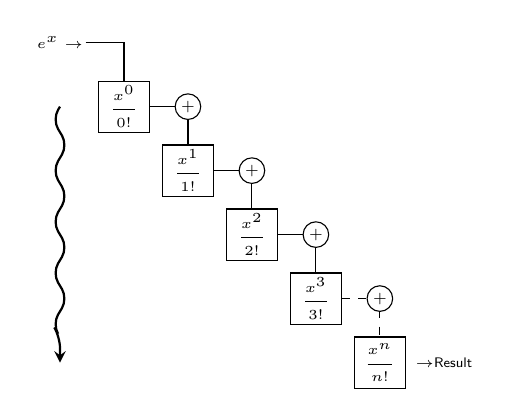
\begin{tikzpicture}[xscale=0.65,yscale=0.65,font=\tiny]
	\newcommand{\Xdisp}{0cm}
	\newcommand{\Ydisp}{0cm}
	% e^x;
	\coordinate [label=center:$e^x\rightarrow$] (exequals) at (\Xdisp-0.75cm,\Ydisp+0.75cm);
	% Single-threaded flow chart.
	\draw (\Xdisp-0.25cm,\Ydisp+0.75cm) -- (\Xdisp+0.5cm,\Ydisp+0.75cm) -- (\Xdisp+0.5cm,\Ydisp);
	\draw (\Xdisp,\Ydisp) rectangle (\Xdisp+1.0cm,\Ydisp-1.0cm);
	\coordinate [label=center:$\dfrac{x^0}{0!}$] (Term0ST) at (\Xdisp+0.5cm,\Ydisp-0.5cm);

	\renewcommand{\Xdisp}{1.25cm}
	\renewcommand{\Ydisp}{-1.25cm}
	\draw (\Xdisp-0.25cm,\Ydisp+0.75cm) -- (\Xdisp+0.5cm,\Ydisp+0.75cm) -- (\Xdisp+0.5cm,\Ydisp);
	\draw (\Xdisp,\Ydisp) rectangle (\Xdisp+1.0cm,\Ydisp-1.0cm);
	\coordinate [label=center:$\dfrac{x^1}{1!}$] (Term1ST) at (\Xdisp+0.5cm,\Ydisp-0.5cm);
	\filldraw[fill=white] (\Xdisp+0.5cm,\Ydisp+0.75cm) circle (0.25cm);
	\coordinate [label=center:$+$] (plusTerm1ST) at (\Xdisp+0.5cm,\Ydisp+0.75cm);

	\renewcommand{\Xdisp}{2.5cm}
	\renewcommand{\Ydisp}{-2.5cm}
	\draw (\Xdisp-0.25cm,\Ydisp+0.75cm) -- (\Xdisp+0.5cm,\Ydisp+0.75cm) -- (\Xdisp+0.5cm,\Ydisp);
	\draw (\Xdisp,\Ydisp) rectangle (\Xdisp+1.0cm,\Ydisp-1.0cm);
	\coordinate [label=center:$\dfrac{x^2}{2!}$] (Term2ST) at (\Xdisp+0.5cm,\Ydisp-0.5cm);
	\filldraw[fill=white] (\Xdisp+0.5cm,\Ydisp+0.75cm) circle (0.25cm);
	\coordinate [label=center:$+$] (plusTerm2ST) at (\Xdisp+0.5cm,\Ydisp+0.75cm);

	\renewcommand{\Xdisp}{3.75cm}
	\renewcommand{\Ydisp}{-3.75cm}
	\draw (\Xdisp-0.25cm,\Ydisp+0.75cm) -- (\Xdisp+0.5cm,\Ydisp+0.75cm) -- (\Xdisp+0.5cm,\Ydisp);
	\draw (\Xdisp,\Ydisp) rectangle (\Xdisp+1.0cm,\Ydisp-1.0cm);
	\coordinate [label=center:$\dfrac{x^3}{3!}$] (Term3ST) at (\Xdisp+0.5cm,\Ydisp-0.5cm);
	\filldraw[fill=white] (\Xdisp+0.5cm,\Ydisp+0.75cm) circle (0.25cm);
	\coordinate [label=center:$+$] (plusTerm3ST) at (\Xdisp+0.5cm,\Ydisp+0.75cm);

	\renewcommand{\Xdisp}{5cm}
	\renewcommand{\Ydisp}{-5cm}
	\draw[dashed] (\Xdisp-0.25cm,\Ydisp+0.75cm) -- (\Xdisp+0.5cm,\Ydisp+0.75cm) -- (\Xdisp+0.5cm,\Ydisp);
	\draw (\Xdisp,\Ydisp) rectangle (\Xdisp+1.0cm,\Ydisp-1.0cm);
	\coordinate [label=center:$\dfrac{x^n}{n!}$] (TermnST) at (\Xdisp+0.5cm,\Ydisp-0.5cm);
	\filldraw[fill=white] (\Xdisp+0.5cm,\Ydisp+0.75cm) circle (0.25cm);
	\coordinate [label=center:$+$] (plusTermnST) at (\Xdisp+0.5cm,\Ydisp+0.75cm);
	% Result
	\coordinate [label=right:$\rightarrow$\textsf{Result}] (ResultST) at (\Xdisp+1.0cm,\Ydisp-0.5cm);
	% Thread.
	\draw[thick, rounded corners, ->, >=stealth] (-0.75cm,-0.5cm) -- (-0.9cm,-0.75cm) -- (-0.6cm,-1.25cm) -- (-0.9cm,-1.75cm) -- (-0.6cm,-2.25cm) -- (-0.9cm,-2.75cm) -- (-0.6cm,-3.25cm) -- (-0.9cm,-3.75cm) -- (-0.6cm,-4.25cm) -- (-0.9cm,-4.75cm) -- (-0.75cm,-5.0cm) -- (-0.75cm,-5.5cm);
\end{tikzpicture}
\end{figure}
\end{frame}
\subsection{Task Parallelism}
\begin{frame}{Task Parallelism}
	\begin{itemize}
	\item Different operations need to be performed that are independent of each other
	\item Example: Summation of terms in a power series
	\end{itemize}
\end{frame}
\begin{frame}{Task Parallelism}
\begin{figure}
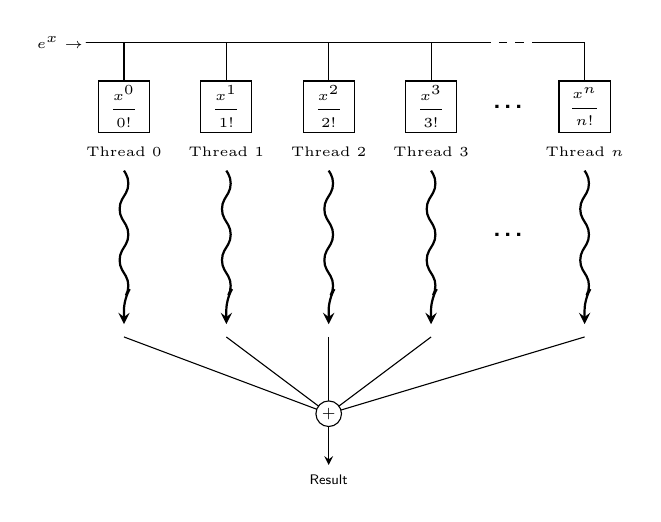
\begin{tikzpicture}[xscale=0.65,yscale=0.65,font=\tiny]
	\newcommand{\Xdisp}{0cm}
	\newcommand{\Ydisp}{0cm}
	% e^x;
	\coordinate [label=center:$e^x\rightarrow$] (exequals) at (\Xdisp-0.75cm,\Ydisp+0.75cm);
	% Single-threaded flow chart.
	\draw (-0.25cm,\Ydisp+0.75cm) -- (\Xdisp+0.5cm,\Ydisp+0.75cm) -- (\Xdisp+0.5cm,\Ydisp);
	\draw (\Xdisp,\Ydisp) rectangle (\Xdisp+1.0cm,\Ydisp-1.0cm);
	\coordinate [label=center:$\dfrac{x^0}{0!}$] (Term0MT) at (\Xdisp+0.5cm,\Ydisp-0.5cm);

	\renewcommand{\Xdisp}{2cm}
	\draw (-0.25cm,\Ydisp+0.75cm) -- (\Xdisp+0.5cm,\Ydisp+0.75cm) -- (\Xdisp+0.5cm,\Ydisp);
	\draw (\Xdisp,\Ydisp) rectangle (\Xdisp+1.0cm,\Ydisp-1.0cm);
	\coordinate [label=center:$\dfrac{x^1}{1!}$] (Term1MT) at (\Xdisp+0.5cm,\Ydisp-0.5cm);

	\renewcommand{\Xdisp}{4cm}
	\draw (-0.25cm,\Ydisp+0.75cm) -- (\Xdisp+0.5cm,\Ydisp+0.75cm) -- (\Xdisp+0.5cm,\Ydisp);
	\draw (\Xdisp,\Ydisp) rectangle (\Xdisp+1.0cm,\Ydisp-1.0cm);
	\coordinate [label=center:$\dfrac{x^2}{2!}$] (Term2MT) at (\Xdisp+0.5cm,\Ydisp-0.5cm);

	\renewcommand{\Xdisp}{6cm}
	\draw (-0.25cm,\Ydisp+0.75cm) -- (\Xdisp+0.5cm,\Ydisp+0.75cm) -- (\Xdisp+0.5cm,\Ydisp);
	\draw (\Xdisp,\Ydisp) rectangle (\Xdisp+1.0cm,\Ydisp-1.0cm);
	\coordinate [label=center:$\dfrac{x^3}{3!}$] (Term3MT) at (\Xdisp+0.5cm,\Ydisp-0.5cm);

	% Dots.
	\coordinate [label=center:\textsf{{\Large ...}}] (Dots1) at (8cm,\Ydisp-0.5cm);
	\coordinate [label=center:\textsf{{\Large ...}}] (Dots2) at (8cm,\Ydisp-3cm);

	\renewcommand{\Xdisp}{9cm}
	\draw (-0.25cm,\Ydisp+0.75cm) -- (\Xdisp-1.5cm,\Ydisp+0.75cm);
	\draw[dashed] (\Xdisp-1.5cm,\Ydisp+0.75cm) -- (\Xdisp-0.5cm,\Ydisp+0.75cm);
	\draw (\Xdisp-0.5cm,\Ydisp+0.75cm) -- (\Xdisp+0.5cm,\Ydisp+0.75cm) -- (\Xdisp+0.5cm,\Ydisp);
	\draw (\Xdisp,\Ydisp) rectangle (\Xdisp+1.0cm,\Ydisp-1.0cm);
	\coordinate [label=center:$\dfrac{x^n}{n!}$] (TermnMT) at (\Xdisp+0.5cm,\Ydisp-0.5cm);

	% Thread numbers.
	\foreach \x/\t in {0.5cm/0,2.5cm/1,4.5cm/2,6.5cm/3,9.5cm/n}
		\coordinate [label=below:Thread $\t$] (Thread\t) at (\x,-1.1cm);
	% Threads.
	\foreach \x in {0.5cm,2.5cm,4.5cm,6.5cm,9.5cm}
		\draw[thick, rounded corners, ->, >=stealth] (\x+0cm,-1.75cm) -- (\x+0.15cm,-2cm) -- (\x-0.15cm,-2.5cm) -- (\x+0.15cm,-3cm) -- (\x-0.15cm,-3.5cm) -- (\x+0.15cm,-4cm) -- (\x+0cm,-4.25cm) -- (\x+0cm,-4.75cm);
	% Summation lines.
	\foreach \x in {0.5cm,2.5cm,4.5cm,6.5cm,9.5cm}
		\draw (\x,-5cm) -- (4.5cm,-6.5cm);
	% Result.
	\draw[->, >=stealth] (4.5cm,-6.5cm) -- (4.5cm,-7.5cm);
	\coordinate [label=below:\textsf{Result}] (ResultMT) at (4.5cm,-7.5cm);
	% Summation.
	\filldraw[fill=white] (4.5cm,-6.5cm) circle (0.25cm);
	\coordinate [label=center:$+$] (PlusSign) at (4.5cm,-6.5cm);
\end{tikzpicture}
%\caption{Task--parallelism}
%\label{fig:Task-Parallelism}
\end{figure}
\end{frame}
\subsection{Data Parallelism}
\begin{frame}{Data Parallelism}
	\begin{itemize}
	\item Same operation needs to be performed on multiple data items
	\item Example: Multiplication of a scalar with matrix
	\end{itemize}
\end{frame}
\begin{frame}{Data Parallelism}
\begin{figure}
\centering
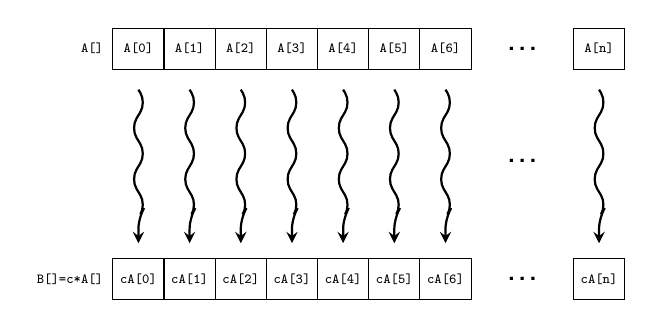
\begin{tikzpicture}[xscale=0.65,yscale=0.65,font=\tiny]
	\newcommand{\Xdisp}{0cm}
	\newcommand{\Ydisp}{0cm}
	% Array A.
	\coordinate [label=left:\texttt{A[]}] (ArrayA) at (\Xdisp,\Ydisp+0.4cm);
	\foreach \x in {0cm,1cm,2cm,3cm,4cm,5cm,6cm,9cm}
		\draw (\x, \Ydisp) rectangle (\x+1cm,\Ydisp+0.8cm);
	\foreach \x/\t in {0.5cm/A[0],1.5cm/A[1],2.5cm/A[2],3.5cm/A[3],4.5cm/A[4],5.5cm/A[5],6.5cm/A[6],9.5cm/A[n]}
		\coordinate [label=center:\texttt{\t}] (Thread\t) at (\x,\Ydisp+0.4cm);
	% Dots.
	\coordinate [label=center:\textsf{{\Large ...}}] (Dots1) at (8cm,\Ydisp+0.4cm);
	% Threads.
	\renewcommand{\Ydisp}{-0.4cm}
	\foreach \x in {0.5cm,1.5cm,2.5cm,3.5cm,4.5cm,5.5cm,6.5cm,9.5cm}
		\draw[thick, rounded corners, ->, >=stealth] (\x+0cm,\Ydisp+0cm) -- (\x+0.15cm,\Ydisp-0.25cm) -- (\x-0.15cm,\Ydisp-0.75cm) -- (\x+0.15cm,\Ydisp-1.25cm) -- (\x-0.15cm,\Ydisp-1.75cm) -- (\x+0.15cm,\Ydisp-2.25cm) -- (\x+0cm,\Ydisp-2.5cm) -- (\x+0cm,\Ydisp-3cm);
	% Dots.
	\coordinate [label=center:\textsf{{\Large ...}}] (Dots2) at (8cm,\Ydisp-1.4cm);
	% Array B.
	\renewcommand{\Ydisp}{-4.5cm}
	\coordinate [label=left:\texttt{B[]=c*A[]}] (ArrayB) at (\Xdisp,\Ydisp+0.4cm);
	\foreach \x in {0cm,1cm,2cm,3cm,4cm,5cm,6cm,9cm}
		\draw (\x, \Ydisp) rectangle (\x+1cm,\Ydisp+0.8cm);
	\foreach \x/\t in {0.5cm/cA[0],1.5cm/cA[1],2.5cm/cA[2],3.5cm/cA[3],4.5cm/cA[4],5.5cm/cA[5],6.5cm/cA[6],9.5cm/cA[n]}
		\coordinate [label=center:\texttt{\t}] (Thread\t) at (\x,\Ydisp+0.4cm);
	% Dots.
	\coordinate [label=center:\textsf{{\Large ...}}] (Dots3) at (8cm,\Ydisp+0.4cm);
\end{tikzpicture}
%\caption{Data--parallelism}
%\label{fig:Data-Parallelism}
\end{figure}
\end{frame}

% How GPUs work?
\subsection{How GPUs Work?}
\begin{frame}{CPU Versus GPU}
	\begin{itemize}
	\item GPUs have rapidly evolved in the last decade
	\item A GPU is typically 5--10 times faster than a similarly priced CPU
	\item Lots of small processors or cores called \textit{shader processors} or \textit{shader} for short
	\item A GPU core is optimised to do only a handful of operations
	\item A CPU core is capable of doing much more
	\item Goal: Use GPU for suitable problems to accelerate processing
	\end{itemize}
\end{frame}
\begin{frame}{CPU Versus GPU}
\begin{figure}[here]
%\centerline{\includegraphics[]{GPGPU}}
\centering
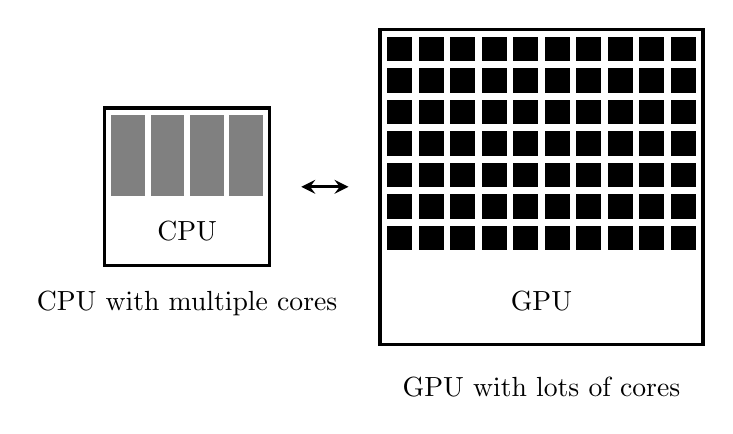
\begin{tikzpicture}
	\draw[very thick] (0cm, 0cm) rectangle (2.1cm, 2cm);
	\foreach \x in {0.1cm,0.6cm,1.1cm, 1.6cm}
		\filldraw[gray, thick] (\x, 0.9cm) rectangle (\x+0.4cm, 1.9cm);
	\coordinate [label=above:CPU] (CPU) at (1.05cm,0.2cm);
	\coordinate [label=below:CPU with multiple cores] (Multi Core CPU) at (1.05cm,-0.2cm);
	
	\draw[very thick, <->, >=stealth] (2.5cm, 1cm) -- (3.1cm, 1cm);
	
	\draw[very thick] (3.5cm, -1cm) rectangle (7.6cm, 3cm);
		\foreach \x in {3.6cm,4cm,4.4cm,4.8cm,5.2cm,5.6cm,6cm,6.4cm,6.8cm,7.2cm}
			\foreach \y in {0.2cm,0.6cm,1cm,1.4cm,1.8cm,2.2cm,2.6cm}
				\filldraw (\x, \y) rectangle (\x+0.3cm, \y+.3cm);
	\coordinate [label=above:GPU] (GPU) at (5.55cm,-0.7cm);
	\coordinate [label=below:GPU with lots of cores] (Multi Core GPU) at (5.55cm,-1.3cm);		
\end{tikzpicture}
%\caption{GPGPU Computing.}
%\label{nVidiaGPGPUfig}
\end{figure}
\end{frame}
% OpenCL and CUDA
\section{Comparison of CUDA and OpenCL}
\subsection{GPU Programming APIs}
\begin{frame}{GPU Programming APIs}
	\begin{itemize}
	\item CUDA (Compute Unified Device Architecture) is the GPU programming API by nVidia exclusive to nVidia hardware
	\item OpenCL (Open Computing Library) is an open source API specification by the khronos group
	\item nVidia and AMD both provide an implementation of OpenCL
	\end{itemize}
\end{frame}
\subsection{OpenCL}
\begin{frame}{OpenCL}
	\begin{itemize}
	\item Hardware Independent: Can work with any GPU
	\item Can even run in emulation mode on CPU if no GPU present
	\item Less intuitive than CUDA but only choice if you don't have nVidia GPU
	\item Less robust than CUDA and some bugs but nothing too serious
	\end{itemize}
\end{frame}
\subsection{CUDA}
\begin{frame}{CUDA}
	\begin{itemize}
	\item Must have an nVidia GPU
	\item Easier to get started
	\item More robust than OpenCL
	\item Good choice for nVidia GPU owners
	\end{itemize}
\end{frame}

% Basics of GPU Programming
\section{Basics of GPU Programming}
\subsection{A Simple Program}
\begin{frame}{A Simple Program}
	\begin{itemize}
	\item Sequence of execution:
		\begin{itemize}
		\item[1.] Allocate CPU (host) memory (RAM) for input and output data
		\item[2.] Allocate GPU (device) memory for input and output data
		\item[3.] Copy input data from host to device
		\item[4.] Execute the `kernel' function that runs on device
		\item[5.] Copy output data from device back to host
		\item[6.] Display or save output
		\item[7.] Cleanup
		\end{itemize}
	\end{itemize}
\end{frame}
\subsection{Where to Get Started?}
\begin{frame}{Where to Get Started?}
	\begin{itemize}
	\item Templates are available for both CUDA and OpenCL
	\item If you don't own a GPU then install OpenCL
	\item Start working with simple programs
	\item \url{supercomputingblog.com} is a great place
	\item We're also here to help
	\end{itemize}
\end{frame}

\section{Performance Analysis}
\subsection{1D Spatial}
\begin{frame}{1D Spatial}
\begin{figure}[H]
\vspace{-0.4cm}
\centering
	\begin{tikzpicture}[xscale=0.5,yscale=0.5]
		\DrawAxes{size}{time~(sec)}
		\GridOn
		\TicksOn
		\XAxisText{0.0391cm/2^8}{}{}{0.625cm/2^{12}}{1.25cm/2^{13}}{2.48cm/2^{14}}{}{ 5cm/2^{15}}{10cm/2^{16}=65536}
		\YAxisText{0cm/0}{0.5cm/1.145}{1cm/2.29}{2cm/4.58}{3cm/6.87}{4cm/9.16}{5cm/11.45}{6cm/13.74}{7cm/16.03}
		\YAxisText{8cm/18.32}{9cm/20.61}{10cm/22.9}{}{}{}{}{}{}
		% 1D spatial with 1024 time steps
		\draw[line width=1pt,color=red!40!yellow] (0.039cm,0.16cm) -- (0.078cm,0.14cm) -- (0.16cm,0.19cm) -- (0.31cm,0.24cm) -- (0.63cm,0.44cm) -- (1.3cm,0.68cm) -- (2.5cm,1.2cm) -- (3.8cm,1.6cm) -- ( 5cm,3.4cm) -- (10cm,8.6cm);
		\draw[line width=1pt,color=red!10!yellow] (0.039cm,0.017cm) -- (0.078cm,0.017cm) -- (0.16cm,0.039cm) -- (0.31cm,0.061cm) -- (0.63cm,0.11cm) -- (1.3cm,0.21cm) -- (2.5cm,0.45cm) -- (3.8cm,0.66cm) -- ( 5cm,1.1cm) -- (10cm,2.4cm);
		\draw[line width=1pt,color=blue] (0.039cm,0.0061cm) -- (0.078cm,0.0087cm) -- (0.16cm,0.024cm) -- (0.31cm,0.044cm) -- (0.63cm,0.079cm) -- (1.3cm,0.21cm) -- (2.5cm,0.5cm) -- (3.8cm,0.75cm) -- ( 5cm, 1cm) -- (10cm, 2cm);
		\draw[line width=1pt,color=blue!30!white] (0.039cm,0.026cm) -- (0.078cm,0.026cm) -- (0.16cm,0.048cm) -- (0.31cm,0.066cm) -- (0.63cm,0.12cm) -- (1.3cm,0.2cm) -- (2.5cm,0.46cm) -- (3.8cm,0.57cm) -- ( 5cm,1.3cm) -- (10cm,2.4cm);
		\draw[line width=1pt,color=gray!70!white] (0.039cm,0.26cm) -- (0.078cm,0.28cm) -- (0.16cm,0.38cm) -- (0.31cm,0.57cm) -- (0.63cm,0.87cm) -- (1.3cm,1.4cm) -- (2.5cm,2.6cm) -- (3.8cm,3.7cm) -- ( 5cm,4.9cm) -- (10cm,9.7cm);
		\draw[line width=1pt,color=pink] (0.039cm,0.33cm) -- (0.078cm,0.34cm) -- (0.16cm,0.49cm) -- (0.31cm,0.56cm) -- (0.63cm,0.77cm) -- (1.3cm,1.4cm) -- (2.5cm,2.5cm) -- (3.8cm,4.9cm) -- ( 5cm,7.1cm) -- (10cm,10cm);
		\draw[line width=1pt,color=red!70!black] (0.039cm,0.18cm) -- (0.078cm,0.1cm) -- (0.16cm,0.1cm) -- (0.31cm,0.1cm) -- (0.63cm,0.11cm) -- (1.3cm,0.12cm) -- (2.5cm,0.14cm) -- (3.8cm,0.15cm) -- ( 5cm,0.17cm) -- (10cm,0.24cm);
		\draw[line width=1pt,color=red] (0.039cm,0.21cm) -- (0.078cm,0.2cm) -- (0.16cm,0.21cm) -- (0.31cm,0.21cm) -- (0.63cm,0.21cm) -- (1.3cm,0.22cm) -- (2.5cm,0.23cm) -- (3.8cm,0.26cm) -- ( 5cm,0.28cm) -- (10cm,0.34cm);
		\draw[line width=1pt,color=green!50!black] (0.039cm,0.045cm) -- (0.078cm,0.048cm) -- (0.16cm,0.047cm) -- (0.31cm,0.053cm) -- (0.63cm,0.062cm) -- (1.3cm,0.083cm) -- (2.5cm,0.1cm) -- (3.8cm,0.12cm) -- ( 5cm,0.12cm) -- (10cm,0.2cm);
		\draw[line width=1pt,color=green] (0.039cm,0.39cm) -- (0.078cm,0.38cm) -- (0.16cm,0.36cm) -- (0.31cm,0.37cm) -- (0.63cm,0.36cm) -- (1.3cm,0.39cm) -- (2.5cm,0.41cm) -- (3.8cm,0.45cm) -- ( 5cm,0.46cm) -- (10cm,0.55cm);
		\DrawLegendRight
	\end{tikzpicture}
\label{fig:Peformance-comparison:1DSpatial}
\end{figure}
\end{frame}
\subsection{1D Spatial for Smaller Array Sizes}
\begin{frame}{1D Spatial for Smaller Array Sizes}
\begin{figure}[H]
\vspace{-0.4cm}
\centering
	\begin{tikzpicture}[xscale=0.5,yscale=0.5]
		\DrawAxes{size}{time~(sec)}
		\GridOn
		\TicksOn
		\XAxisText{0.313cm/2^8}{0.625cm/2^{9}}{1.25cm/2^{10}}{2.5cm/2^{11}}{ 5cm/2^{12}(4096)}{10cm/2^{13}(8192)}{}{}{}{}{}
		\YAxisText{0.00cm/0.00}{0.50cm/0.16}{1.00cm/0.32}{1.50cm/0.48}{2.00cm/0.64}{2.50cm/0.80}{3.00cm/0.96}{3.50cm/1.12}{4.00cm/1.28}
		\YAxisText{4.50cm/1.44}{5.00cm/1.60}{5.50cm/1.76}{6.00cm/1.92}{6.50cm/2.08}{7.00cm/2.24}{7.50cm/2.40}{8.00cm/2.56}{8.50cm/2.72}
		\YAxisText{9.00cm/2.88}{9.50cm/3.04}{10.00cm/3.20}{}{}{}{}{}{}
		% 1D spatial upto size=2^13 with 1024 time steps
		\draw[line width=1pt,color=red!40!yellow] (0.31cm,1.1cm) -- (0.63cm, 1cm) -- (1.3cm,1.4cm) -- (2.5cm,1.7cm) -- ( 5cm,3.1cm) -- (10cm,4.9cm);
		\draw[line width=1pt,color=red!10!yellow] (0.31cm,0.13cm) -- (0.63cm,0.13cm) -- (1.3cm,0.28cm) -- (2.5cm,0.44cm) -- ( 5cm,0.78cm) -- (10cm,1.5cm);
		\draw[line width=1pt,color=blue] (0.31cm,0.044cm) -- (0.63cm,0.063cm) -- (1.3cm,0.17cm) -- (2.5cm,0.31cm) -- ( 5cm,0.56cm) -- (10cm,1.5cm);
		\draw[line width=1pt,color=blue!30!white] (0.31cm,0.19cm) -- (0.63cm,0.19cm) -- (1.3cm,0.34cm) -- (2.5cm,0.47cm) -- ( 5cm,0.84cm) -- (10cm,1.4cm);
		\draw[line width=1pt,color=gray!70!white] (0.31cm,1.9cm) -- (0.63cm, 2cm) -- (1.3cm,2.8cm) -- (2.5cm,4.1cm) -- ( 5cm,6.3cm) -- (10cm,10cm);
		\draw[line width=1pt,color=pink] (0.31cm,2.3cm) -- (0.63cm,2.4cm) -- (1.3cm,3.5cm) -- (2.5cm, 4cm) -- ( 5cm,5.5cm) -- (10cm,9.7cm);
		\draw[line width=1pt,color=red!70!black] (0.31cm,1.3cm) -- (0.63cm,0.72cm) -- (1.3cm,0.73cm) -- (2.5cm,0.74cm) -- ( 5cm,0.77cm) -- (10cm,0.84cm);
		\draw[line width=1pt,color=red] (0.31cm,1.5cm) -- (0.63cm,1.4cm) -- (1.3cm,1.5cm) -- (2.5cm,1.5cm) -- ( 5cm,1.5cm) -- (10cm,1.6cm);
		\draw[line width=1pt,color=green!50!black] (0.31cm,0.32cm) -- (0.63cm,0.34cm) -- (1.3cm,0.34cm) -- (2.5cm,0.38cm) -- ( 5cm,0.45cm) -- (10cm,0.59cm);
		\draw[line width=1pt,color=green] (0.31cm,2.8cm) -- (0.63cm,2.7cm) -- (1.3cm,2.6cm) -- (2.5cm,2.6cm) -- ( 5cm,2.6cm) -- (10cm,2.8cm);
		\DrawLegendRight
	\end{tikzpicture}
\label{fig:Peformance-comparison:1DSpatialSmallerArraySizes}
\end{figure}
\end{frame}
\subsection{2D Spatial}
\begin{frame}{2D Spatial}
\begin{figure}[H]
\vspace{-0.4cm}
\centering
	\begin{tikzpicture}[xscale=0.5,yscale=0.5]
		\DrawAxes{size}{time~(sec)}
		\GridOn
		\TicksOn
		\XAxisText{0.313cm/32^2}{1.25cm/128^2}{2.5cm/256^2}{3.75cm/384^2}{ 5cm/512^2}{6.25cm/640^2}{7.5cm/768^2}{8.75cm/896^2}{10cm/1024^2}
		\YAxisText{0.00cm/0}{1.00cm/60}{2.00cm/120}{3.00cm/180}{4.00cm/240}{5.00cm/300}{6.00cm/360}{7.00cm/420}{8.00cm/480}
		\YAxisText{9.00cm/540}{10.00cm/600}{}{}{}{}{}{}{}
		% 2D spatial all plots with 256 time steps
		\draw[line width=1pt,color=red!40!yellow] (0.31cm,0.019cm) -- (0.63cm,0.025cm) -- (1.3cm,0.048cm) -- (2.5cm,0.2cm) -- (3.8cm,0.59cm) -- ( 5cm,1.2cm) -- (6.3cm,2.1cm) -- (7.5cm,3.3cm) -- (8.8cm,4.4cm) -- (10cm, 6cm);
		\draw[line width=1pt,color=red!10!yellow] (0.31cm,0.00082cm) -- (0.63cm,0.0038cm) -- (1.3cm,0.02cm) -- (2.5cm,0.3cm) -- (3.8cm,0.41cm) -- ( 5cm,2.5cm) -- (6.3cm,2.5cm) -- (7.5cm,5.2cm) -- (8.8cm,5.9cm) -- (10cm,9.8cm);
		\draw[line width=1pt,color=blue] (0.31cm,0.00087cm) -- (0.63cm,0.0033cm) -- (1.3cm,0.017cm) -- (2.5cm,0.32cm) -- (3.8cm,0.5cm) -- ( 5cm,2.1cm) -- (6.3cm,2.7cm) -- (7.5cm,4.4cm) -- (8.8cm,5.6cm) -- (10cm,8.5cm);
		\draw[line width=1pt,color=blue!30!white] (0.31cm,0.0032cm) -- (0.63cm,0.0062cm) -- (1.3cm,0.022cm) -- (2.5cm,0.13cm) -- (3.8cm,0.37cm) -- ( 5cm,2.3cm) -- (6.3cm,2.3cm) -- (7.5cm,4.8cm) -- (8.8cm,5.4cm) -- (10cm,9.2cm);
		\draw[line width=1pt,color=gray!70!white] (0.31cm,0.0093cm) -- (0.63cm,0.011cm) -- (1.3cm,0.017cm) -- (2.5cm,0.049cm) -- (3.8cm,0.091cm) -- ( 5cm,0.17cm) -- (6.3cm,0.24cm) -- (7.5cm,0.36cm) -- (8.8cm,0.5cm) -- (10cm,0.66cm);
		\draw[line width=1pt,color=pink] (0.31cm,0.013cm) -- (0.63cm,0.013cm) -- (1.3cm,0.017cm) -- (2.5cm,0.046cm) -- (3.8cm,0.095cm) -- ( 5cm,0.18cm) -- (6.3cm,0.25cm) -- (7.5cm,0.36cm) -- (8.8cm,0.45cm) -- (10cm,0.66cm);
		\draw[line width=1pt,color=red!70!black] (0.31cm,0.0022cm) -- (0.63cm,0.0027cm) -- (1.3cm,0.0035cm) -- (2.5cm,0.0078cm) -- (3.8cm,0.014cm) -- ( 5cm,0.023cm) -- (6.3cm,0.034cm) -- (7.5cm,0.049cm) -- (8.8cm,0.066cm) -- (10cm,0.085cm);
		\draw[line width=1pt,color=red] (0.31cm,0.0067cm) -- (0.63cm,0.0067cm) -- (1.3cm,0.0078cm) -- (2.5cm,0.012cm) -- (3.8cm,0.02cm) -- ( 5cm,0.03cm) -- (6.3cm,0.043cm) -- (7.5cm,0.058cm) -- (8.8cm,0.075cm) -- (10cm,0.097cm);
		\draw[line width=1pt,color=green!50!black] (0.31cm,0.0012cm) -- (0.63cm,0.0014cm) -- (1.3cm,0.0021cm) -- (2.5cm,0.0068cm) -- (3.8cm,0.013cm) -- ( 5cm,0.024cm) -- (6.3cm,0.035cm) -- (7.5cm,0.051cm) -- (8.8cm,0.068cm) -- (10cm,0.089cm);
		\draw[line width=1pt,color=green] (0.31cm,0.005cm) -- (0.63cm,0.005cm) -- (1.3cm,0.0067cm) -- (2.5cm,0.011cm) -- (3.8cm,0.019cm) -- ( 5cm,0.03cm) -- (6.3cm,0.043cm) -- (7.5cm,0.06cm) -- (8.8cm,0.081cm) -- (10cm,0.1cm);
		\DrawLegendRight
	\end{tikzpicture}
\label{fig:Peformance-comparison:Spatial}
\end{figure}
\end{frame}
\subsection{2D Temporal}
\begin{frame}{2D Temporal}
\begin{figure}[H]
\vspace{-0.4cm}
\centering
	\begin{tikzpicture}[xscale=0.5,yscale=0.5]
		\DrawAxes{steps}{time~(sec)}
		\GridOn
		\TicksOn
		\XAxisText{0.05cm/25}{1cm/}{2cm/1000}{3cm/}{4cm/2000}{5cm/}{6cm/3000}{7cm/}{8cm/4000}
		\XAxisText{9cm/}{10cm/5000}{}{}{}{}{}{}{}
		\YAxisText{0.00cm/0}{1.00cm/280}{2.00cm/560}{3.00cm/840}{4.00cm/1120}{5.00cm/1400}{6.00cm/1680}{7.00cm/1960}{8.00cm/2240}
		\YAxisText{9.00cm/2520}{10.00cm/2800}{}{}{}{}{}{}{}
		% ------- 2D temporal with 512^2 size -------
		\draw[line width=1pt,color=red!40!yellow] (0.05cm,0.027cm) -- (0.1cm,0.047cm) -- (0.2cm,0.094cm) -- (0.4cm,0.19cm) -- (0.6cm,0.28cm) -- (0.8cm,0.38cm) -- ( 1cm,0.48cm) -- (1.5cm,0.72cm) -- ( 2cm,0.97cm) -- ( 3cm,1.5cm) -- ( 4cm,1.9cm) -- ( 5cm,2.3cm) -- ( 6cm,2.8cm) -- ( 7cm,3.2cm) -- ( 8cm,3.6cm) -- ( 9cm,4.1cm) -- (10cm,4.5cm);
		\draw[line width=1pt,color=red!10!yellow] (0.05cm,0.052cm) -- (0.1cm,0.11cm) -- (0.2cm,0.21cm) -- (0.4cm,0.4cm) -- (0.6cm,0.6cm) -- (0.8cm,0.8cm) -- ( 1cm, 1cm) -- (1.5cm,1.5cm) -- ( 2cm, 2cm) -- ( 3cm, 3cm) -- ( 4cm, 4cm) -- ( 5cm, 5cm) -- ( 6cm, 6cm) -- ( 7cm, 7cm) -- ( 8cm, 8cm) -- ( 9cm, 9cm) -- (10cm,10cm);
		\draw[line width=1pt,color=blue] (0.05cm,0.046cm) -- (0.1cm,0.076cm) -- (0.2cm,0.15cm) -- (0.4cm,0.29cm) -- (0.6cm,0.44cm) -- (0.8cm,0.6cm) -- ( 1cm,0.73cm) -- (1.5cm,1.1cm) -- ( 2cm,1.4cm) -- ( 3cm,2.1cm) -- ( 4cm,2.8cm) -- ( 5cm,3.4cm) -- ( 6cm, 4cm) -- ( 7cm,4.6cm) -- ( 8cm,5.3cm) -- ( 9cm,5.9cm) -- (10cm,6.3cm);
		\draw[line width=1pt,color=blue!30!white] (0.05cm,0.048cm) -- (0.1cm,0.094cm) -- (0.2cm,0.18cm) -- (0.4cm,0.37cm) -- (0.6cm,0.55cm) -- (0.8cm,0.73cm) -- ( 1cm,0.91cm) -- (1.5cm,1.4cm) -- ( 2cm,1.9cm) -- ( 3cm,2.9cm) -- ( 4cm,3.8cm) -- ( 5cm,4.6cm) -- ( 6cm,5.7cm) -- ( 7cm,6.6cm) -- ( 8cm,7.5cm) -- ( 9cm,8.4cm) -- (10cm,9.3cm);
		\draw[line width=1pt,color=gray!70!white] (0.05cm,0.014cm) -- (0.1cm,0.01cm) -- (0.2cm,0.016cm) -- (0.4cm,0.026cm) -- (0.6cm,0.038cm) -- (0.8cm,0.053cm) -- ( 1cm,0.059cm) -- (1.5cm,0.086cm) -- ( 2cm,0.11cm) -- ( 3cm,0.17cm) -- ( 4cm,0.22cm) -- ( 5cm,0.27cm) -- ( 6cm,0.32cm) -- ( 7cm,0.46cm) -- ( 8cm,0.49cm) -- ( 9cm,0.49cm) -- (10cm,0.53cm);
		\draw[line width=1pt,color=pink] (0.05cm,0.0099cm) -- (0.1cm,0.011cm) -- (0.2cm,0.017cm) -- (0.4cm,0.028cm) -- (0.6cm,0.04cm) -- (0.8cm,0.051cm) -- ( 1cm,0.063cm) -- (1.5cm,0.092cm) -- ( 2cm,0.12cm) -- ( 3cm,0.18cm) -- ( 4cm,0.24cm) -- ( 5cm,0.29cm) -- ( 6cm,0.35cm) -- ( 7cm,0.41cm) -- ( 8cm,0.47cm) -- ( 9cm,0.52cm) -- (10cm,0.58cm);
		\draw[line width=1pt,color=red!70!black] (0.05cm,0.003cm) -- (0.1cm,0.0025cm) -- (0.2cm,0.0029cm) -- (0.4cm,0.0037cm) -- (0.6cm,0.0045cm) -- (0.8cm,0.0053cm) -- ( 1cm,0.0062cm) -- (1.5cm,0.0082cm) -- ( 2cm,0.01cm) -- ( 3cm,0.015cm) -- ( 4cm,0.018cm) -- ( 5cm,0.023cm) -- ( 6cm,0.027cm) -- ( 7cm,0.031cm) -- ( 8cm,0.035cm) -- ( 9cm,0.039cm) -- (10cm,0.043cm);
		\draw[line width=1pt,color=red] (0.05cm,0.0068cm) -- (0.1cm,0.0041cm) -- (0.2cm,0.0045cm) -- (0.4cm,0.0054cm) -- (0.6cm,0.0063cm) -- (0.8cm,0.0072cm) -- ( 1cm,0.0083cm) -- (1.5cm,0.011cm) -- ( 2cm,0.013cm) -- ( 3cm,0.017cm) -- ( 4cm,0.022cm) -- ( 5cm,0.027cm) -- ( 6cm,0.031cm) -- ( 7cm,0.036cm) -- ( 8cm,0.04cm) -- ( 9cm,0.045cm) -- (10cm,0.05cm);
		\draw[line width=1pt,color=green!50!black] (0.05cm,0.0029cm) -- (0.1cm,0.0026cm) -- (0.2cm,0.0031cm) -- (0.4cm,0.0039cm) -- (0.6cm,0.0048cm) -- (0.8cm,0.0057cm) -- ( 1cm,0.0066cm) -- (1.5cm,0.0088cm) -- ( 2cm,0.011cm) -- ( 3cm,0.016cm) -- ( 4cm,0.02cm) -- ( 5cm,0.024cm) -- ( 6cm,0.029cm) -- ( 7cm,0.033cm) -- ( 8cm,0.038cm) -- ( 9cm,0.042cm) -- (10cm,0.047cm);
		\draw[line width=1pt,color=green] (0.05cm,0.0045cm) -- (0.1cm,0.0036cm) -- (0.2cm,0.0041cm) -- (0.4cm,0.0051cm) -- (0.6cm,0.006cm) -- (0.8cm,0.0072cm) -- ( 1cm,0.0079cm) -- (1.5cm,0.01cm) -- ( 2cm,0.013cm) -- ( 3cm,0.018cm) -- ( 4cm,0.022cm) -- ( 5cm,0.027cm) -- ( 6cm,0.032cm) -- ( 7cm,0.036cm) -- ( 8cm,0.041cm) -- ( 9cm,0.046cm) -- (10cm,0.051cm);
		\DrawLegendRight
	\end{tikzpicture}
\label{fig:Peformance-comparison:Temporal}
\end{figure}
\end{frame}

\section{GPU Implementation of Cylindrical Cloak}
\subsection{Introduction}
\begin{frame}{Introduction}
	\begin{itemize}
	\item We can see objects when light bounces off them and reach our eyes
	\item If light bends around an object without reflection or scattering then that object will not be visible
	\item Electromagnetic cloak made of metamaterial was proposed by Pendry et. al \cite{PendryShurig-MicrowaveCloak}
	\item An FDTD implementation was developed by Zhao et. al \cite{Radial-Zhao}
	\item A GPU implementation was developed using CUDA
	\end{itemize}
\end{frame}
\subsection{Problem Geometry}
\begin{frame}
\begin{figure}[H]
\centering
\vspace{-0.3cm}
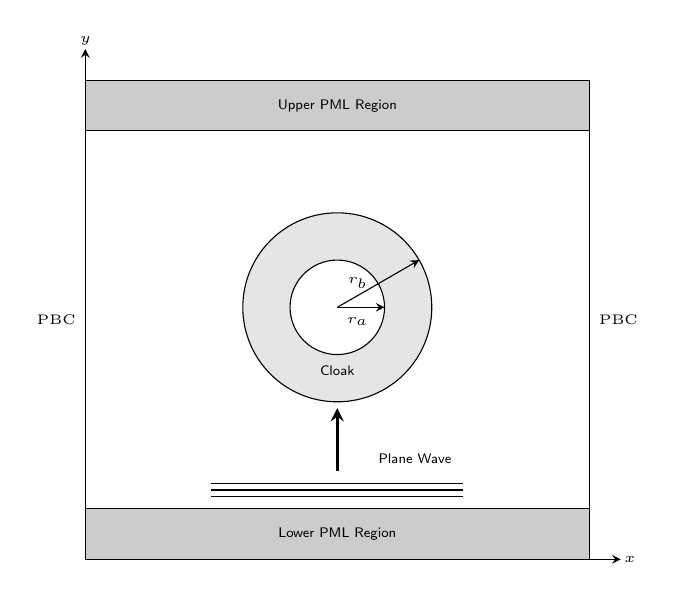
\begin{tikzpicture}[xscale=0.8,yscale=0.8]
	\newcommand{\LeftX}{0cm}
	\newcommand{\MidX}{4cm}
	\newcommand{\RightX}{8cm}
	\newcommand{\PMLw}{0.8cm}
	\newcommand{\DomainY}{6.0cm}
	\newcommand{\SlabStartY}{2.0cm+\PMLw}
	\newcommand{\SlabEndY}{4.0cm+\PMLw}
	% x-axis.
	\draw[->, >=stealth] (\LeftX,0cm) -- (\RightX+0.5cm,0cm);
	\coordinate [label=right:{\tiny $x$}] (x-axis) at (\RightX+0.4cm,0cm);
	% y-axis.
	\draw[->, >=stealth] (\LeftX,0cm) -- (\LeftX,2*\PMLw+\DomainY+0.5cm);
	\coordinate [label=above:{\tiny $y$}] (y-axis) at (\LeftX,2*\PMLw+\DomainY+0.4cm);
	% PBCs.
	\coordinate [label=right:{\tiny PBC}] (PBCright) at (\RightX,\PMLw+3.0cm);
	\coordinate [label=left:{\tiny PBC}] (PBCleft) at (\LeftX,\PMLw+3.0cm);
	% Lower PML Region.
	\draw[fill=gray!40!white] (\LeftX,0cm) rectangle (\RightX,\PMLw);
	\coordinate [label=center:{\tiny \textsf{Lower PML Region}}] (LowerPML) at (\MidX,0.4cm);
	% Solution Region.
	\draw (\LeftX,\PMLw) rectangle (\RightX,\PMLw+\DomainY);
	% Upper PML Region.
	\draw[fill=gray!40!white] (\LeftX,\PMLw+\DomainY) rectangle (\RightX,2*\PMLw+\DomainY);
	\coordinate [label=center:{\tiny \textsf{Upper PML Region}}] (UpperPML) at (\MidX,\PMLw+\DomainY+0.4cm);
	% Cloaking shell.
	\draw[fill=gray!20!white] (4cm,4cm) circle (1.5cm);
	\draw[fill=white] (4cm,4cm) circle (0.75cm);
	\coordinate [label=center:{\tiny \textsf{Cloak}}] (Cloak) at (\MidX,3cm);
	\draw[->, >=stealth] (\MidX,4cm) -- (\MidX+0.75cm,4cm);
	\draw[->, >=stealth] (\MidX,4cm) -- (\MidX+1.3005cm,4.75cm);
	\coordinate [label=below:{\tiny $r_a$}] (ra) at (\MidX+0.325cm,4cm);
	\coordinate [label=above:{\tiny $r_b$}] (rb) at (\MidX+0.325cm,4.15cm);
	% Plane wave.
	\draw (\LeftX+2.0cm,\PMLw+0.2cm) -- (\RightX-2.0cm, \PMLw+0.2cm);
	\draw (\LeftX+2.0cm,\PMLw+0.3cm) -- (\RightX-2.0cm, \PMLw+0.3cm);
	\draw (\LeftX+2.0cm,\PMLw+0.4cm) -- (\RightX-2.0cm, \PMLw+0.4cm);
	\draw[line width=1.1pt, ->, >=stealth] (\MidX,\PMLw+0.6cm) -- (\MidX,\PMLw+1.6cm);
	\coordinate [label=right:{\tiny \textsf{Plane Wave}}] (PlaneWave) at (\MidX+0.5cm,\PMLw+0.8cm);
\end{tikzpicture}
\label{fig:2D-Cloak-Geometry}
\end{figure}
\end{frame}
\subsection{Cloak Simulation: Ez Under Steady State}
\begin{frame}{Cloak Simulation: Ez Under Steady State}
\begin{figure}[H]
\centering
\vspace{-0.325cm}
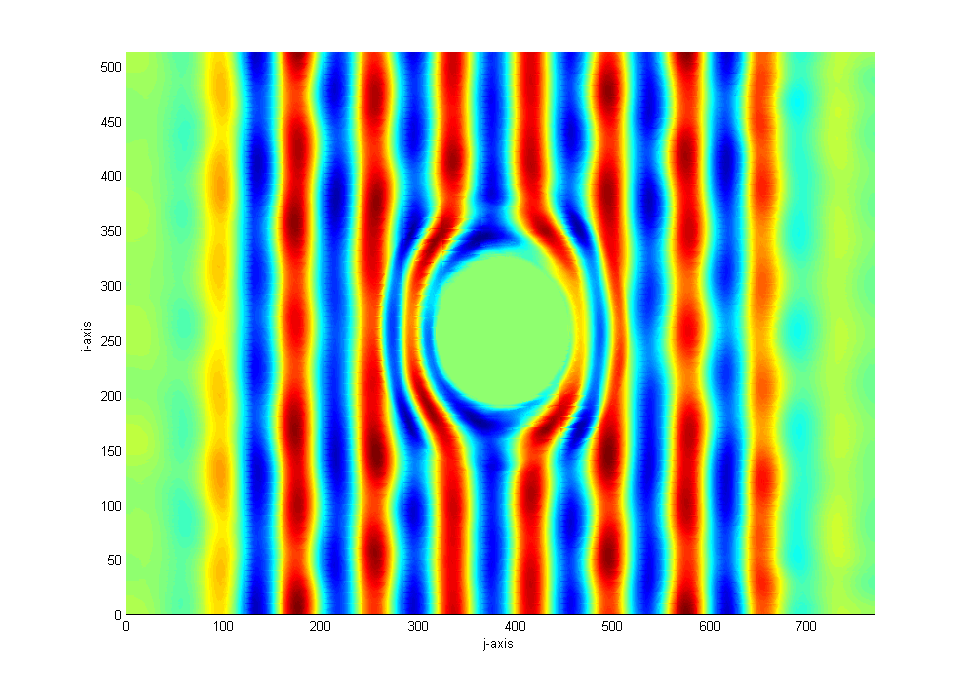
\includegraphics[scale=0.325]{Figures/FigCh05_Ez_Cloak_SteadyStateLossless.png}
\label{fig:Ez-Cloak-SteadyStateLossless}
\end{figure}
\end{frame}

\section{Conclusion}
\begin{frame}{Conclusion}
	\begin{itemize}
	\item GPU programming is an emerging new technology
	\item Building your own GPU--based supercomputer is exciting!
	\item Has its limitations
	\item Cloud computing and virtual supercomputing
	\item Can pursue a degree in high performance computing
	\end{itemize}
\end{frame}

\subsubsection{References}
\begin{frame}[t,allowframebreaks]{References}
	\nocite{*}
	\bibliographystyle{ieeetr} %plain, ieeetr
	{\tiny \bibliography{GPGPUref}}
\end{frame}
\end{document}